\documentclass[12pt,a4paper]{article}
\usepackage{mathptmx} % added for time new roman font
\usepackage[left=0.5in,right=0.5in,top=1in,bottom=1in]{geometry}
\usepackage[latin1]{inputenc}
\usepackage{amsmath}
\usepackage{amsfonts}
\usepackage{amssymb}
\usepackage{graphicx}
\usepackage{float}
\usepackage{booktabs}
\usepackage{parskip} % remove all the paragraph indents


\usepackage{setspace}
\usepackage[colorlinks=true]{hyperref}
\usepackage{textcomp} 
\usepackage{multicol} 

\usepackage{mathtools}          %loads amsmath as well added for the piece wise function
\DeclarePairedDelimiter\Floor\lfloor\rfloor
\DeclarePairedDelimiter\Ceil\lceil\rceil

 
\newcounter{NumberInTable}
\newcommand{\LTNUM}{\stepcounter{NumberInTable}{(\theNumberInTable)}}

\newcommand{\Laplace}[1]{\ensuremath{\mathcal{L}{\left[#1\right]}}}
\newcommand{\InvLap}[1]{\ensuremath{\mathcal{L}^{-1}{\left[#1\right]}}}
\renewcommand{\textuparrow}{$\uparrow$}

\begin{document}
	
	\large{}
	\title{\vspace{-2cm}Lecture Notes, Topic-8}
	\date{}
	\maketitle
	
	\section*{Review from previous class}
		\begin{enumerate}
			\item Harmonic excitations of underdamped systems
			\item Frequency response
		\end{enumerate}
	
	\section*{Objectives for today's class}
	\begin{enumerate}
		\item Base excitations
	\end{enumerate}
	
	\section*{Lecture}
	
		\subsection*{Base excitation}

Often, loading is not applied directly to the mass, but rather the mass of the system is excited when the base of mount that it is attached to is excited. This is called base excitation, or sometimes support motion. Examples of base excitation, or where base excitation is considered, include:

\begin{itemize}
\item machines on rubber mounts
\item automobiles excited by the road
\item building under earthquake loading
\item hospital equipment
\end{itemize}

Consider the following system base excited system
\begin{figure}[H]
	\centering
	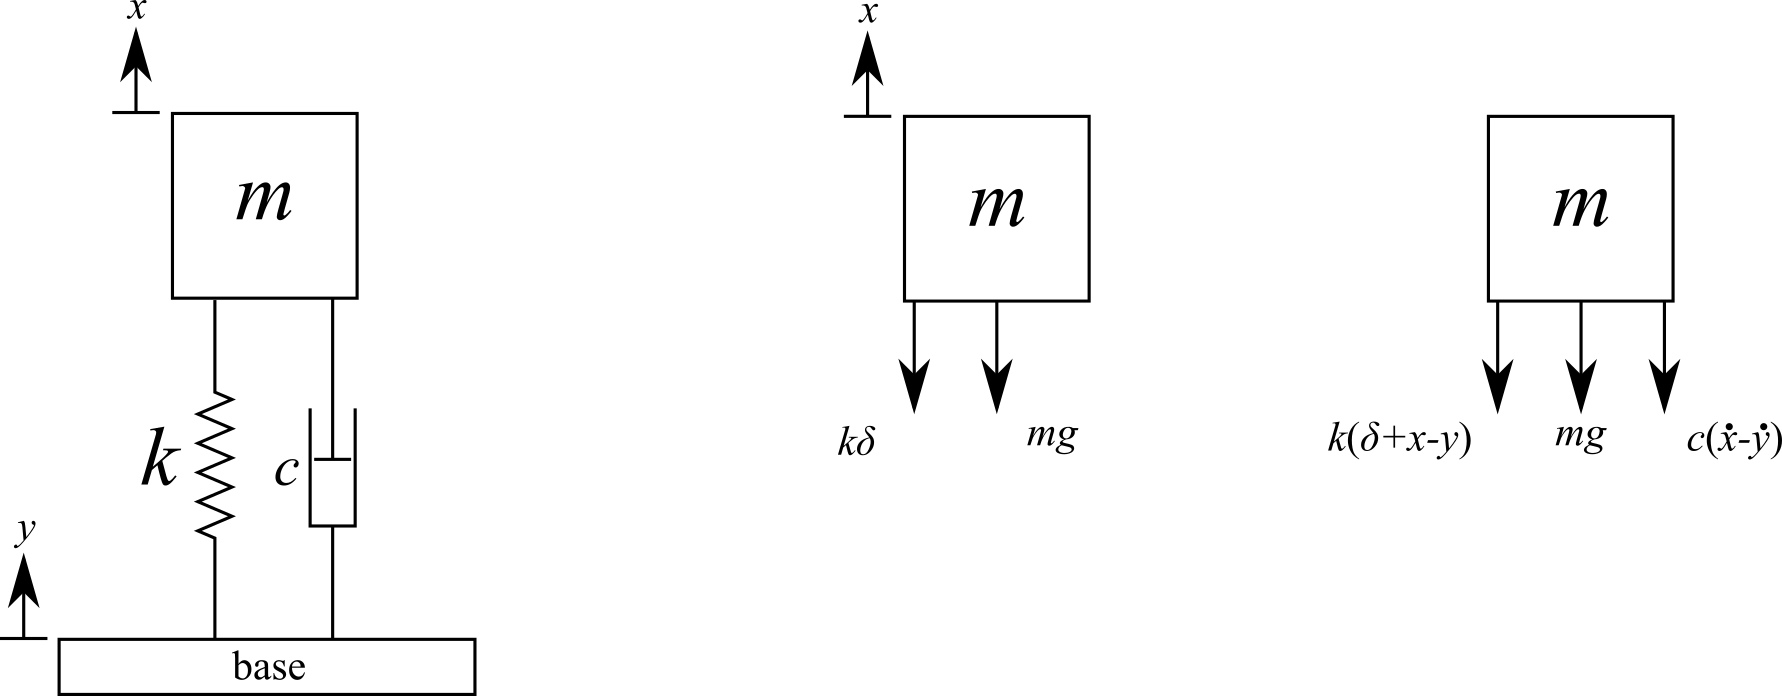
\includegraphics[width=0.8\textwidth]{../../Figures/base_excited_1_DOF_model_and_FBDs.png}
\end{figure}
where $x$ is the displacement of the mass and $y$ is the displacement of the base. \textbf{Note that we consider positive upward here.} The EOM can be constructed the same as before, but now considering that the displacement of the springs and damper is $x-y$.  In the equilibrium state, where a positive $x$ is up and the base displaces down:
\begin{equation}
-k\delta -mg =0
\end{equation}	
Note that these are both negative because the base displacing down ``pulls'' the mass down with a force $k\delta$ (i.e. if you hold the mass and let the base ``fall''). Conversely, the equation for the displaced state is:
\begin{equation}
\sum F_x = -k(\delta + x - y) -mg -c(\dot{x} -\dot{y})
\end{equation}	
Apply Newton's second law about the mass ($m\ddot{x}$) of motion to the sum of forces for the displaced position we get:
\begin{equation}
\sum F_x = m\ddot{x} = -k\delta -kx + ky -mg -c\dot{x} +c\dot{y}
\end{equation}	
applying the equation $-k\delta -mg =0$, and rearrange into the EOM yields:	
\begin{equation}
m\ddot{x} + c\dot{x} + kx = c\dot{y} + ky 
\end{equation}
Now as before we assume a solution for the base excitation, for simplicity we assume
\begin{equation}
y(t) = Y\text{sin}(\omega_b t)
\end{equation}
Taking the derivative of the assume solution yields
\begin{equation}
\dot{y}(t) = Y \omega_b \text{cos}(\omega_b t)
\end{equation}
where $Y$ is the amplitude and $\omega_b$ is the frequency of the base excitation. Adding these terms into our EOM yields:
\begin{equation}
m\ddot{x} + c\dot{x} + kx = c Y \omega_b \text{cos}(\omega_b t)  + k Y\text{sin}(\omega_b t)  
\end{equation}
We can get this in standard form if we divide by $m$ and apply the equations for the critical damping ratio and natural frequency:
\begin{equation}
\ddot{x} + 2 \zeta \omega_n \dot{x} + \omega_n^2x = 2 \zeta \omega_n \omega_b Y \text{cos}(\omega_b t)  + \omega_n^2 Y\text{sin}(\omega_b t)  
\end{equation}
This equation can be related to a spring-mass-damper system with two harmonic inputs, one cos and one sin as shown below:
\begin{equation}
\ddot{x} + 2 \zeta \omega_n \dot{x} + \omega_n^2x = C \text{cos}(\omega_b t)  + D \text{sin}(\omega_b t)  
\end{equation}
where C and D are arbitrary coefficients. For simplicity, let us just consider the steady-state solution as this is often of more importance when designing systems for continuous use. Therefore the above equation can be expressed as:
\begin{equation}
\ddot{x} + 2 \zeta \omega_n \dot{x} + \omega_n^2x = C \text{cos}(\omega_b t)  + D \text{sin}(\omega_b t)  = x_p(t) 
\end{equation}
To solve this equation we will use the linearity of the system and solve for a solution that is the sum of two partial solutions. Resulting in:
\begin{equation}
 x_p(t) = 	x_p^{(1)}(t) + 	x_p^{(2)}(t)  
\end{equation}

 Recall that the steady state solution for a harmonically excited spring-mass-damper can be expressed as $x_p(t) = X\text{cos}(\omega_b t - \phi_1)$. Therefore, for a base excited problem, the forcing function can be expressed as the sum of partial solutions:
\begin{equation}
	C \text{cos}(\omega_b t)  + D \text{sin}(\omega_b t)   = x_p(t) = 	x_p^{(1)}(t) + 	x_p^{(2)}(t) 
\end{equation}
where:
\begin{equation}
	x_p^{(1)}(t) = X^{(1)}\text{cos}(\omega_b t - \phi_1)
\end{equation}
\begin{equation}
	x_p^{(2)}(t) = X^{(2)} \text{sin}(\omega_b t - \phi_1)
\end{equation}
Note that $x_p^{(1)}(t)$ uses a cos term while $x_p^{(1)}(t)$ uses a sin term. Both solutions use $\phi_1$ as the damping term as the phase angle is independent of the excitation amplitude and the sin and cos terms account for the difference in phase. Now, for $x_p^{(1)}(t)$, we use the method of undetermined coefficients to obtain a solution for $x_p^{(1)}(t) = X^{(1)}\text{cos}(\omega_b t - \phi_1)$. This can be as simple as setting $2 \zeta \omega_n \omega_b Y$ equal to $f_0$ from the equation for $X$. We can do this because both terms can be considered a ``driving force''. This results in the equation:
\begin{equation}
	x_p^{(1)}(t) = \frac{2 \zeta \omega_n \omega_b Y}{\sqrt{(\omega_n^2 - \omega_b^2)^2 +  (2\zeta \omega_n \omega_b)^2}}  \text{cos}(\omega_b t - \phi_1)
\end{equation}
where 
\begin{equation}
	\phi_1 = \text{tan}^-1\bigg(\frac{2\zeta \omega_n \omega_b}{\omega_n^2 - \omega_b^2}\bigg)
\end{equation}	
Next, the partial solution associated with $x_p^{(2)}(t) = X^{(2)} \text{sin}(\omega_b t - \phi_1)$ can be obtained using the same method of undetermined coefficients. This results in:
\begin{equation}
	x_p^{(2)}(t) = \frac{\omega_n^2 Y}{\sqrt{(\omega_n^2 - \omega_b^2)^2 +  (2\zeta \omega_n \omega_b)^2}}  \text{sin}(\omega_b t - \phi_1)
\end{equation}
now, as both equation have the same argument $(\omega_b t - \phi_1)$, these can be added as:
\begin{equation}
	x_p(t) = 	x_p^{(1)}(t) + 	x_p^{(2)}(t)
\end{equation}
to obtain:
\begin{equation}
	x_p(t) = 	\omega_n Y   \sqrt{\frac{\omega_n^2 + (2 \zeta \omega_b)^2 }{(\omega_n^2 - \omega_b^2)^2 +  (2\zeta \omega_n \omega_b)^2} }  \text{cos}(\omega_bt - \phi_1 - \phi_2)
\end{equation}
and:
\begin{equation}
	\phi_2 = \text{tan}^-1\bigg(\frac{\omega_n}{2\zeta \omega_b}\bigg)
\end{equation}
where $\phi_2$ is added to account for the cos and sin terms being combined. As before, if we want to investigate how a frequency input will affect the response (frequency response) we can substitute substitute 
\begin{equation}
r=\frac{\omega_b}{\omega_n}
\end{equation} 
into the temporal response to obtain:
\begin{equation}
X = Y \sqrt{\frac{1+(2 \zeta r)^2}{(1-r^2)^2 + (2 \zeta r )^2}} 
\end{equation} 
Next, if we divide by $Y$ we can obtain a normalized expression for the displacement:
\begin{equation}
\frac{X}{Y} = \sqrt{\frac{1+(2 \zeta r)^2}{(1-r^2)^2 + (2 \zeta r )^2}} 
\end{equation} 
Plotting this for several critical damping ratios:
\begin{figure}[H]
	\centering
	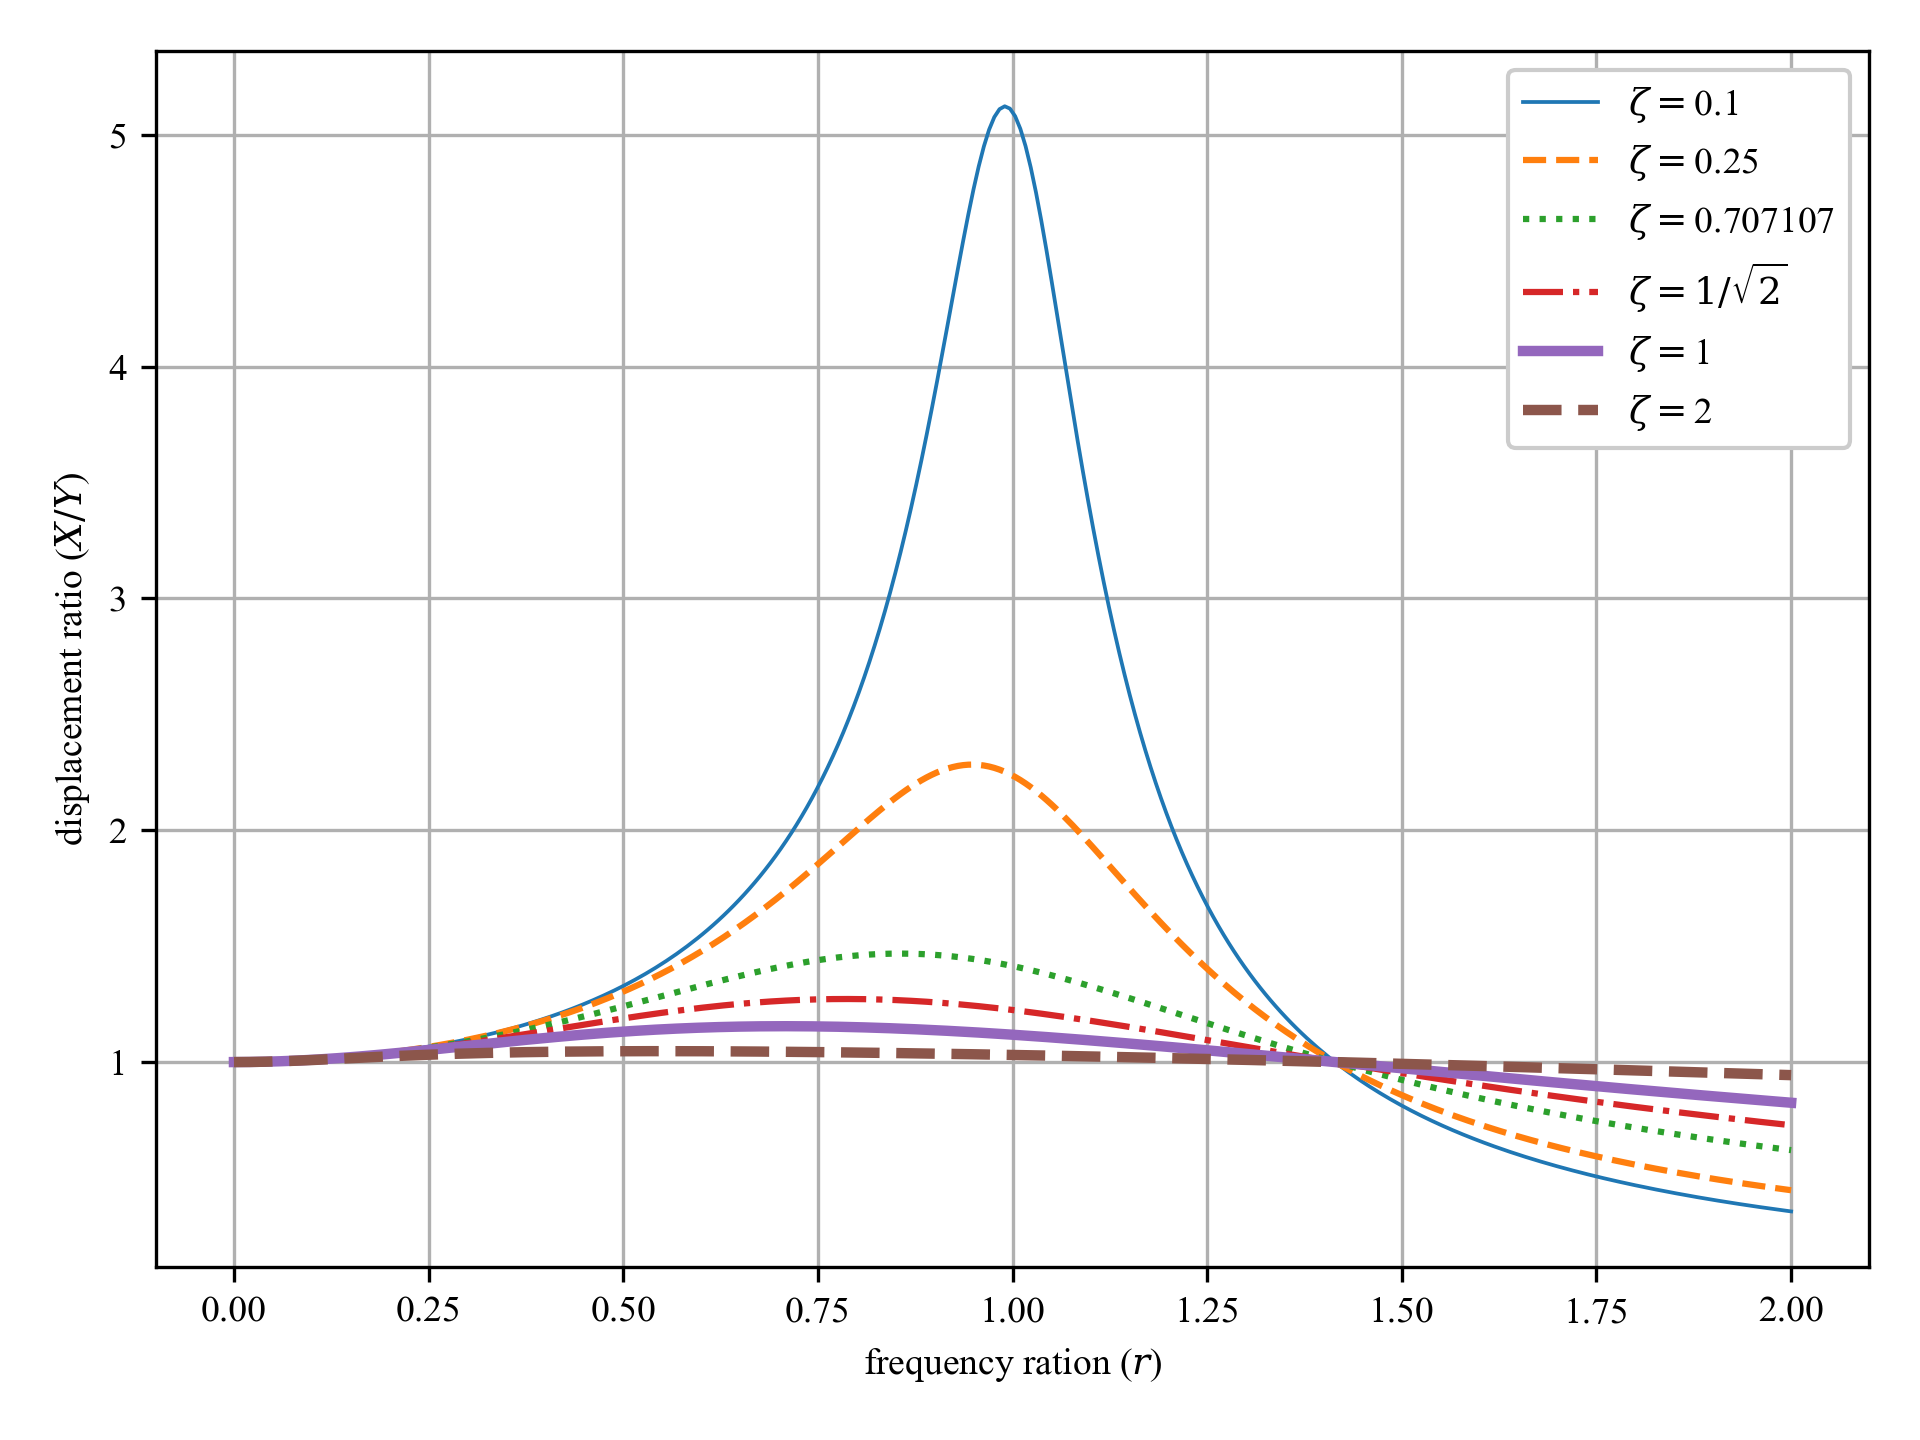
\includegraphics[width=0.8\textwidth]{../../Figures/displacement_transmissibility.png}
\end{figure}
Around resonance, the maximum amount of displacement is transmitted to the mass. Additionally,  the above plot shows that at $r=\sqrt{2}$ the displacement transmissibility $X/Y$ is 1. Note the ``flip'' where overdamped systems have a greater response to excitations after $r=\sqrt{2}$ than do underdamped systems.

For some systems, such as those with weak connections, the force transmitted to the mass is more important than the displacement of the mass. The force transmitted to the mass are the sums of the forces applied by the spring and damper. From the FBD above,
\begin{equation}
F(t) = k(x-y) + c(\dot{x} - \dot{y}) 
\end{equation}
where this force is counteracted by the inertial force of the mass:
\begin{equation}
F(t) = -m\ddot{x}(t)
\end{equation}
Only considering the steady state we found that 
\begin{equation}
	x_p(t) = 	\omega_n Y   \sqrt{\frac{\omega_n^2 + (2 \zeta \omega_b)^2 }{(\omega_n^2 - \omega_b^2)^2 +  (2\zeta \omega_n \omega_b)^2} }  \text{cos}(\omega_bt - \phi_1 - \phi_2)
\end{equation} 
if we differentiate this twice, to obtain $\ddot{x}(t)$ and combine this with $F(t) = -m\ddot{x}(t)$ we get:
\begin{equation}
	F(t) = 	m \omega_b^2 \omega_n Y   \sqrt{\frac{\omega_n^2 + (2 \zeta \omega_b)^2 }{(\omega_n^2 - \omega_b^2)^2 +  (2\zeta \omega_n \omega_b)^2} }  \text{cos}(\omega_bt - \phi_1 - \phi_2)
\end{equation} 
Again applying 
\begin{equation}
	r=\frac{\omega_b}{\omega_n}
\end{equation} 
this becomes:
\begin{equation}
	F(t) = 	F_\text{T} \text{cos}(\omega_bt - \phi_1 - \phi_2)
\end{equation} 
where $F_T$ is the magnitude of the transmitted force and is 
\begin{equation}
	F_\text{T} = kYr^2 \sqrt{\frac{1+(2 \zeta r)^2}{(1-r^2)^2 + (2 \zeta r )^2}} 
\end{equation}
Again, this can be converted to a force transmissibility to provide a normalized response such that:
\begin{equation}
	\frac{F_\text{T}}{kY} = r^2 \sqrt{\frac{1+(2 \zeta r)^2}{(1-r^2)^2 + (2 \zeta r )^2}} 
\end{equation}
Plotting this for several critical damping ratios:
\begin{figure}[H]
	\centering
	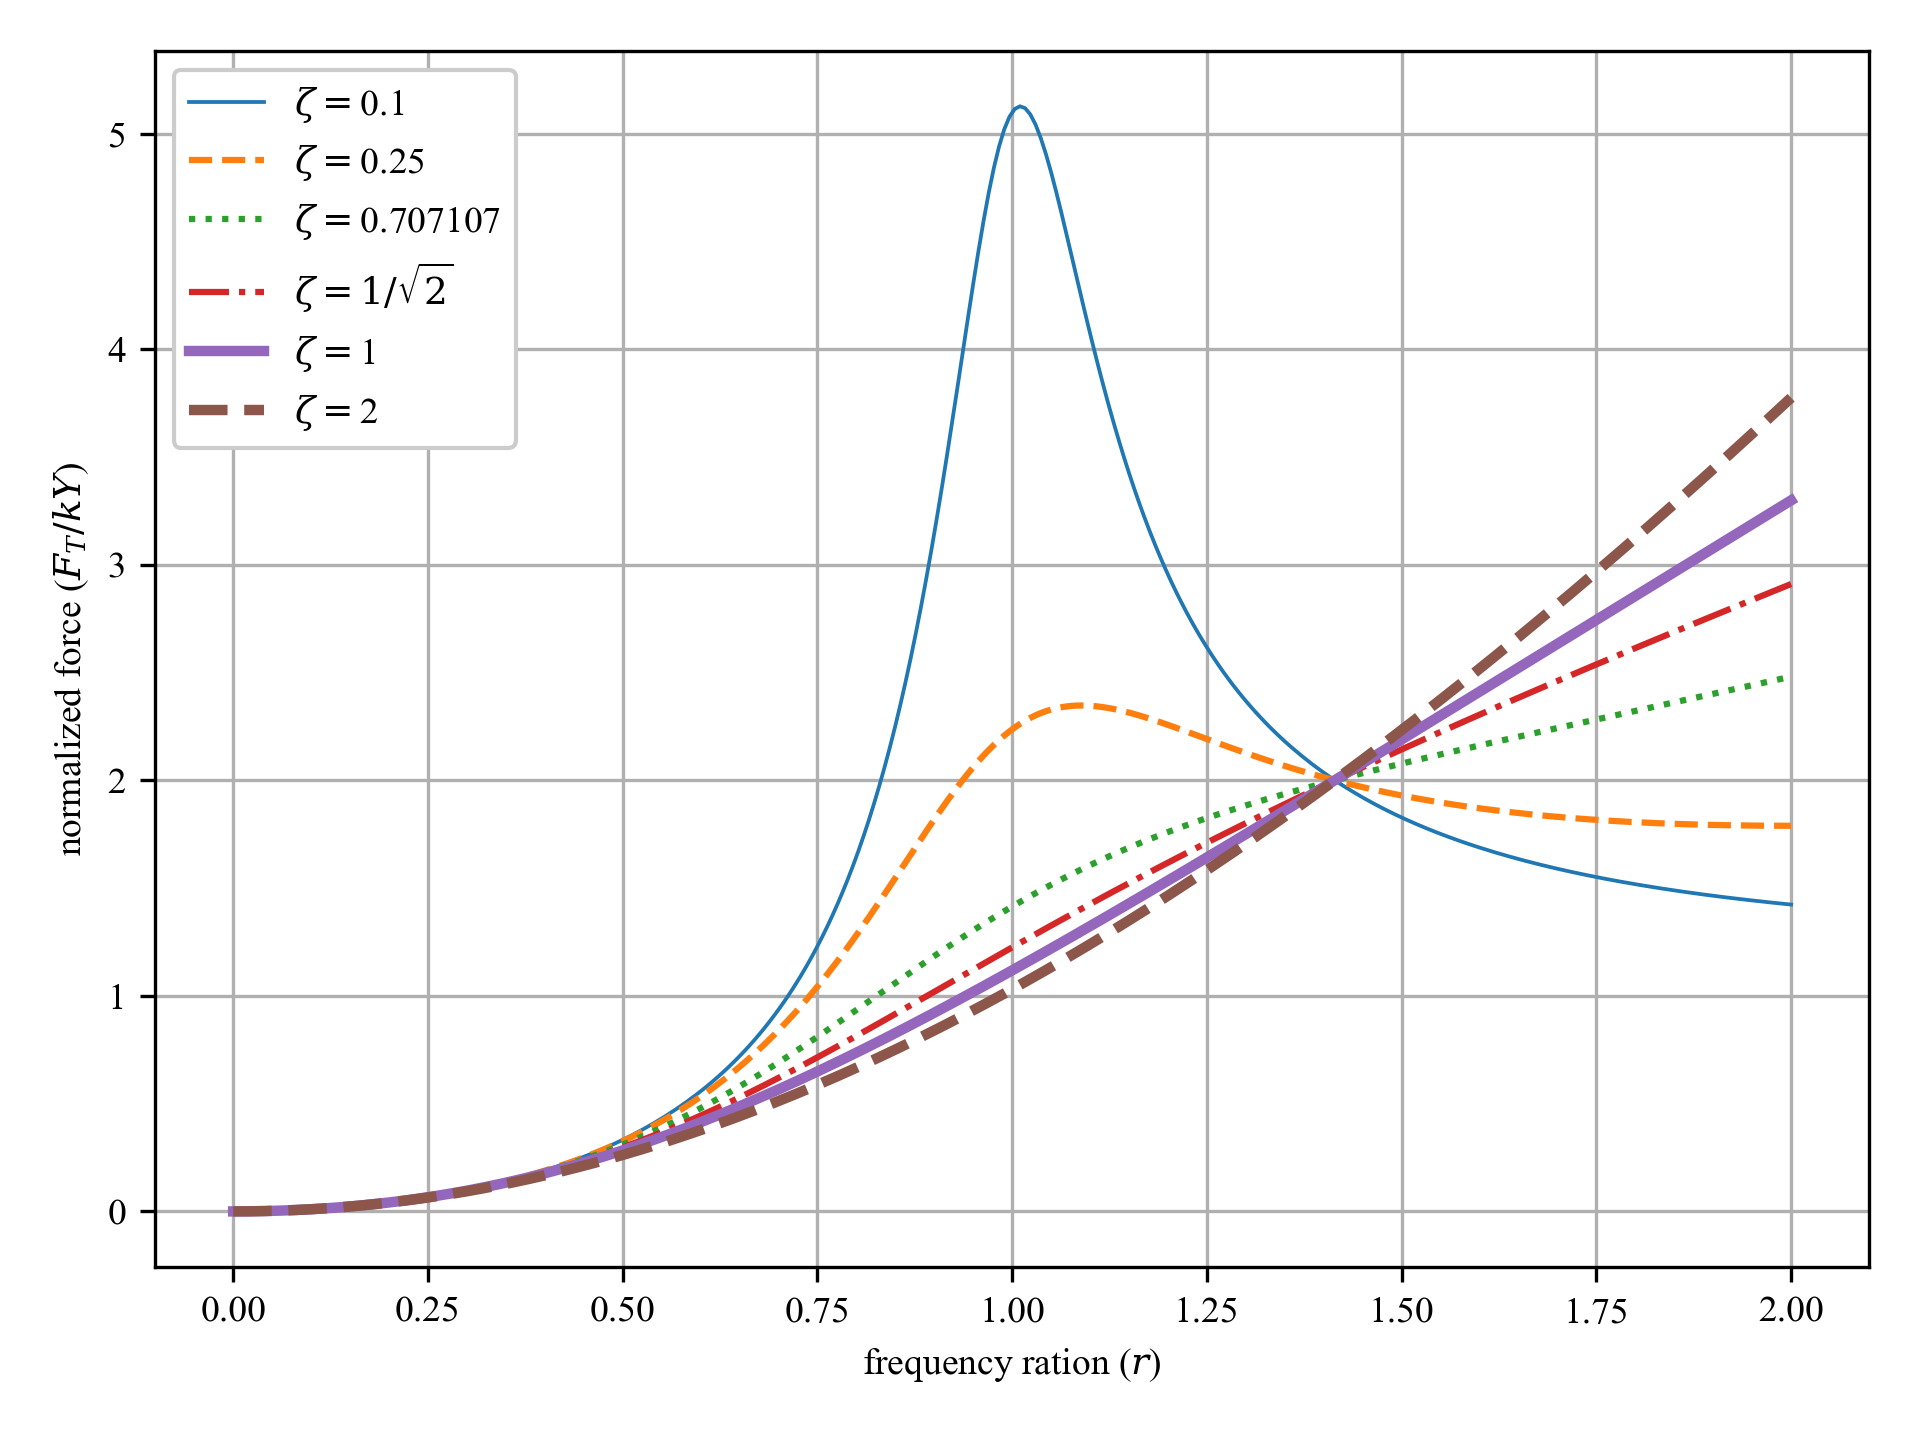
\includegraphics[width=0.8\textwidth]{../../Figures/force_transmissibility.png}
\end{figure}
Again, note the key location $r=\sqrt{2}$. At $r=\sqrt{2}$ the force transmitted to the system is 2 $\frac{F_\text{T}}{kY}$. However, also note that the normalized force does not necessarily fall off for $r$ values greater than $r=\sqrt{2}$.  

		\subsection*{Example 1}

			For a given system 1-DOF excited at the base should the system be excited above or below the natural frequency if the transmitted force is the design limitation? Consider the under damped with $\zeta=0.1$, and the over damped with $\zeta=2$ conditions. 

			\textbf{Solution}
			
			We can plot the transmissibility of both the force and displacement onto one plot. For $\zeta=0.1$
			\begin{figure}[H]
				\centering
				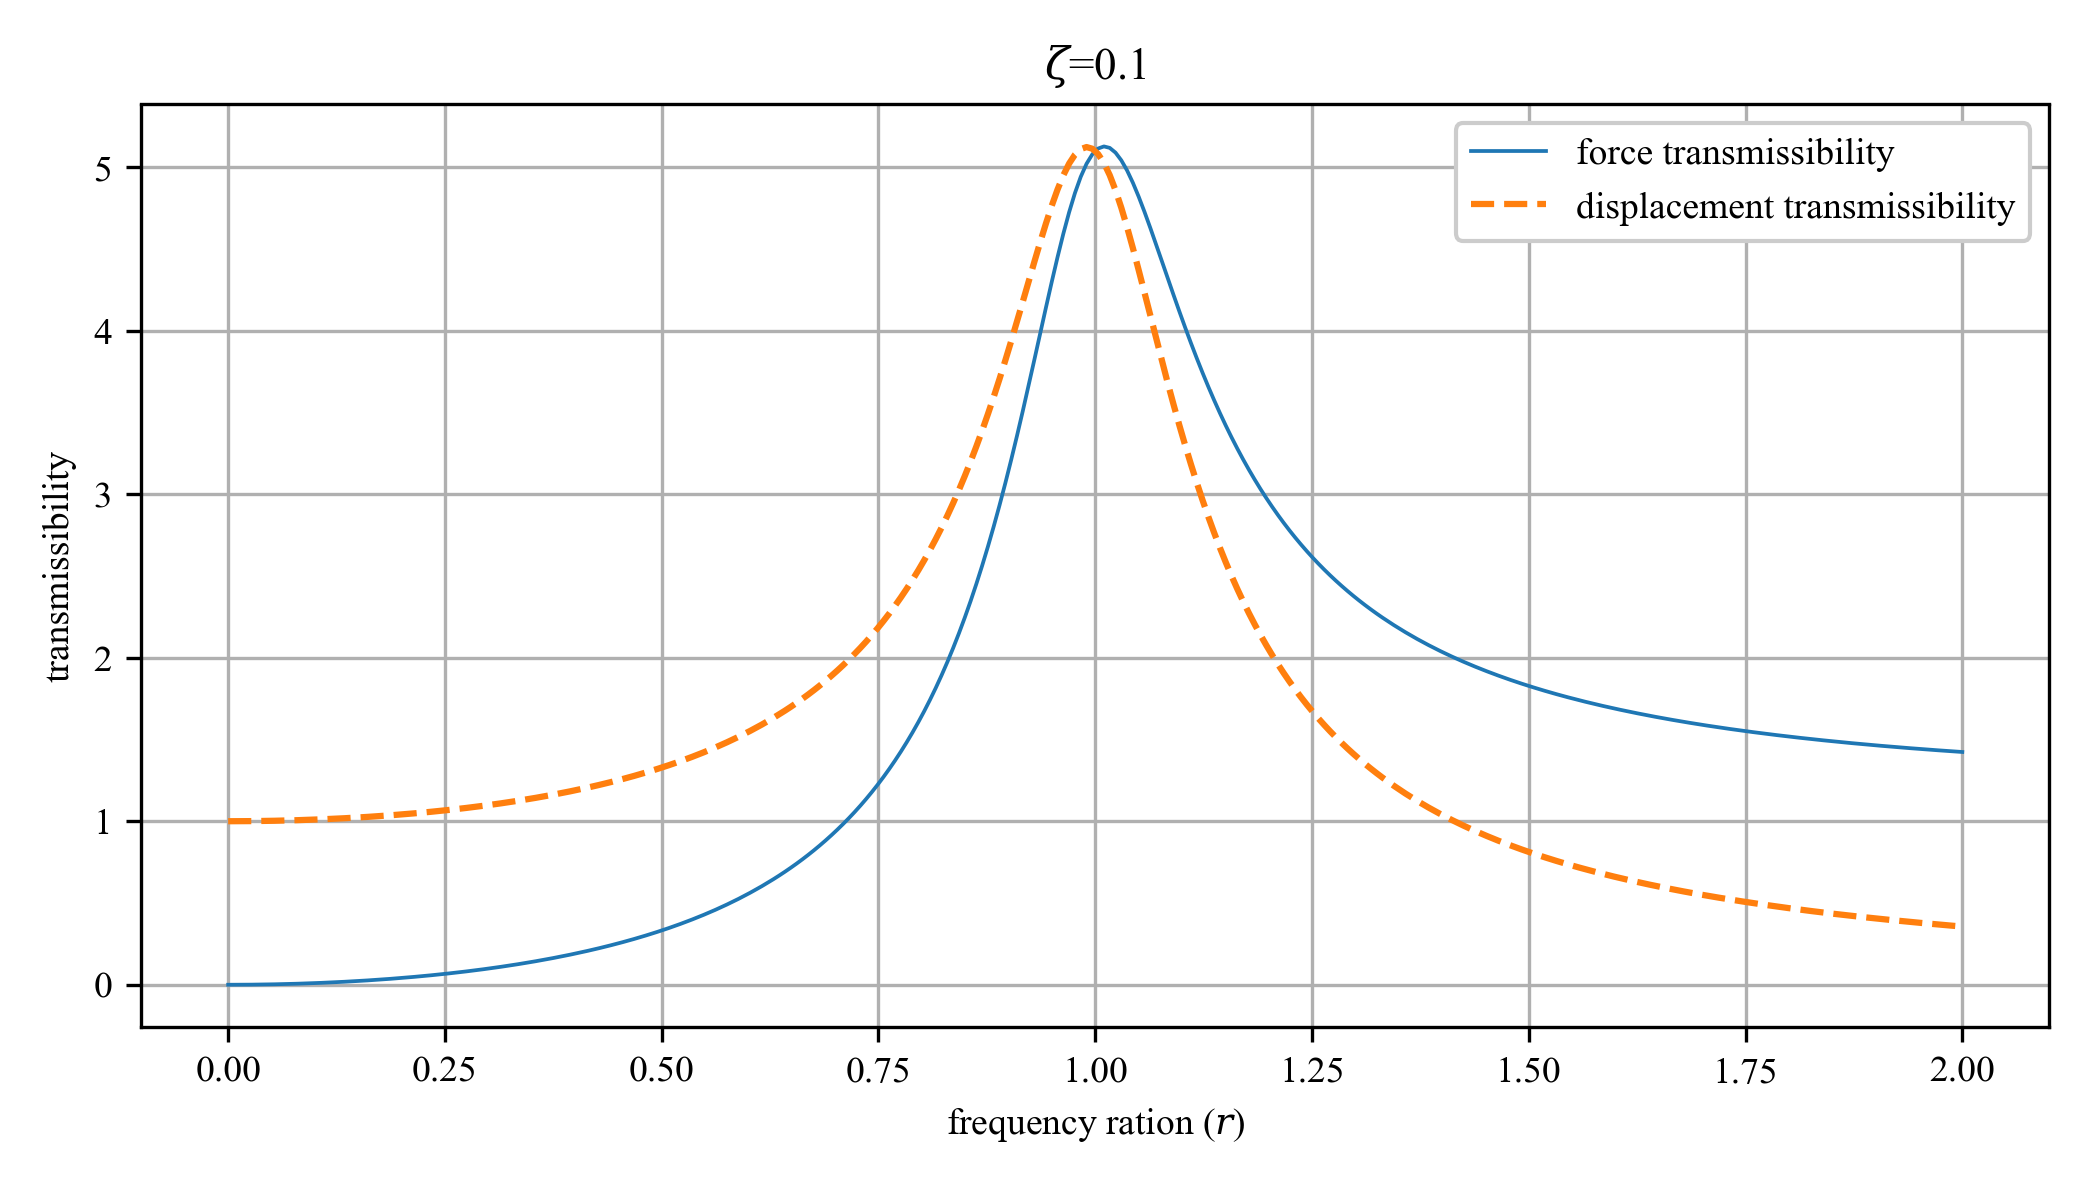
\includegraphics[width=0.8\textwidth]{../../Figures/example_1_force_displacement_transmissibility_1.png}
			\end{figure}
			it is clear that to minimize the force, the system should be driven with a frequency below the natural frequency. Next for  $\zeta=2$
			\begin{figure}[H]
				\centering
				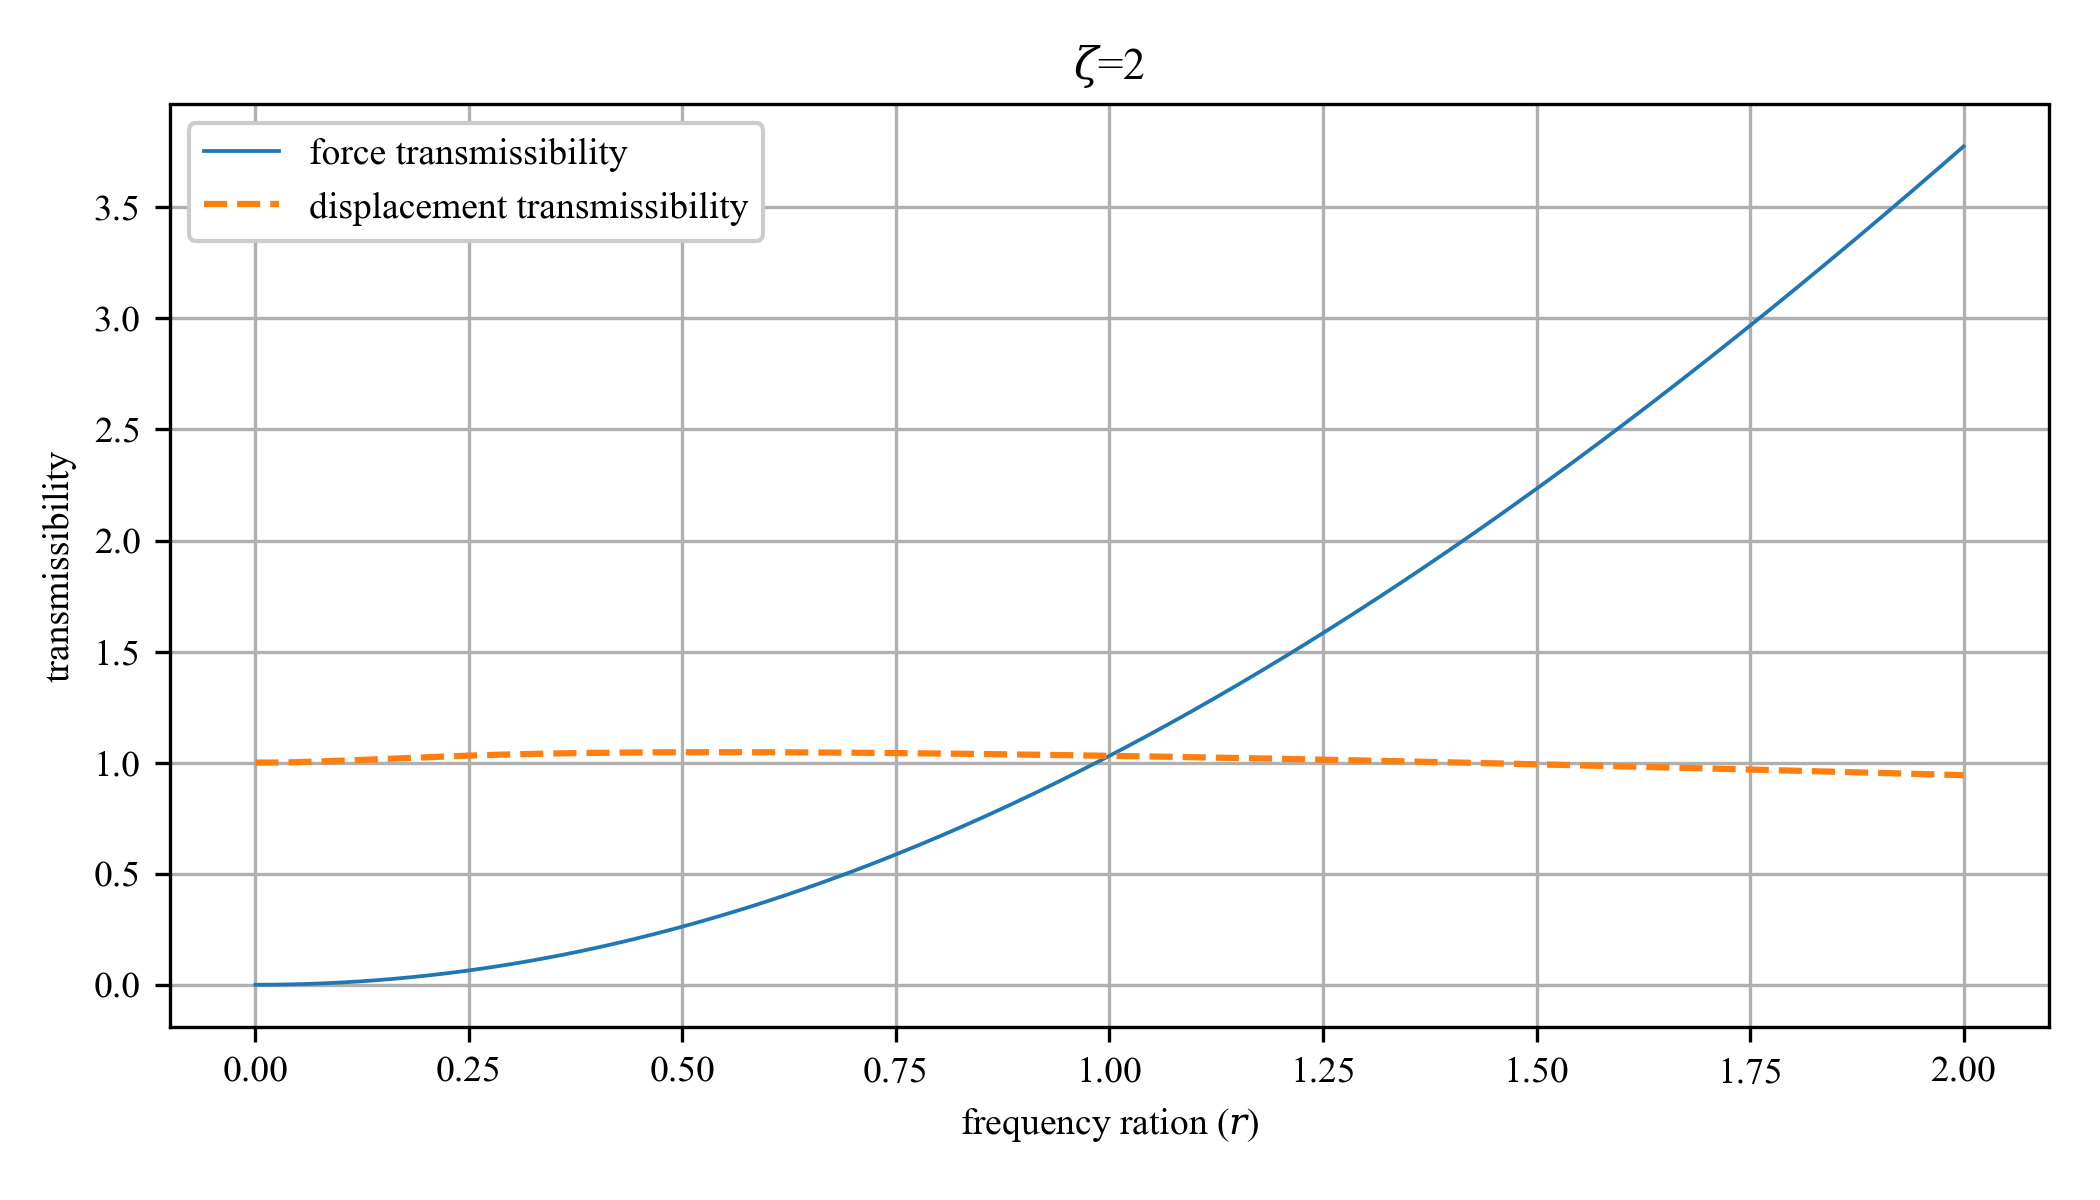
\includegraphics[width=0.8\textwidth]{../../Figures/example_1_force_displacement_transmissibility_2.png}
			\end{figure}			
			it can be seen that the same rationale applies. 
			
		\subsection*{Example 2}
	
			A \textbf{very common} example of base motion is the SDOF model of a vehicle wheel driving over a ``rough'' road as shown below. 
			\begin{figure}[H]
				\centering
				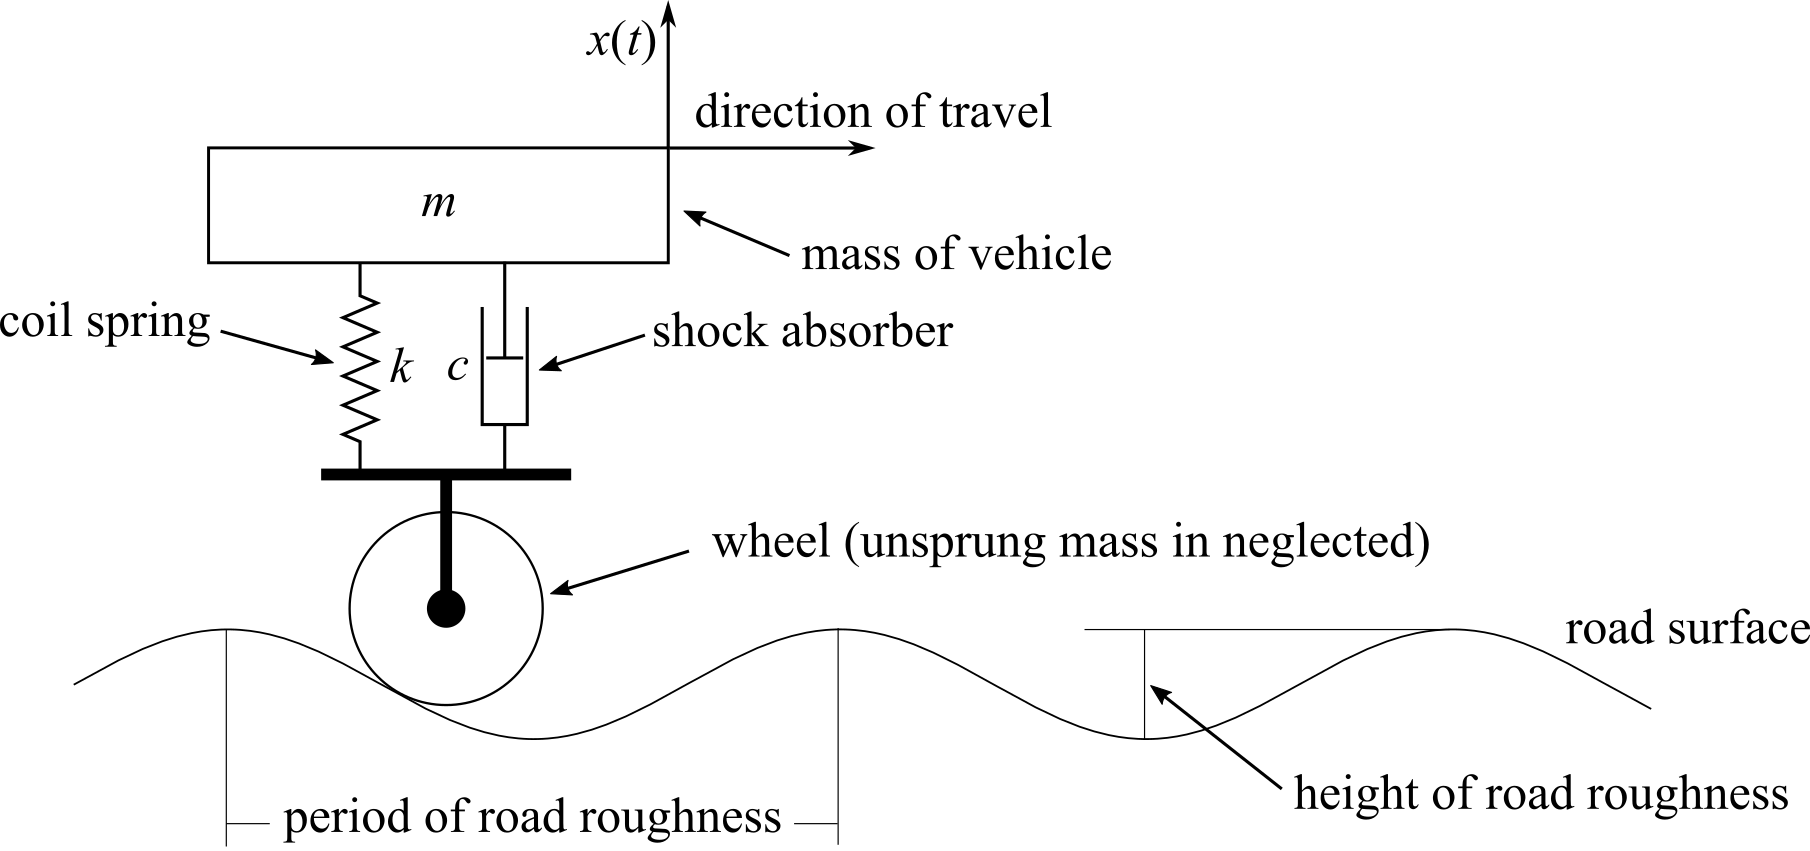
\includegraphics[width=0.8\textwidth]{../../Figures/vehicle_on_road_example.png}
			\end{figure}				
			where $k$ = 400,000 N, $m$ = 1007 kg, and $c$ = 20,000 kg/s. What is the defection experience by the car at $v$ = 20 km/h?
			
			\textbf{Solution}

			The road is applying a base excitation that can be approximated as 
			\begin{equation}
				Y = 0.01 \text{ m}
			\end{equation} 				
			\begin{equation}
				v \text{ m/s} = 20 \text{ km/hr}\Bigg(\frac{1000 \text{ m}}{1 \text {km}}\Bigg) \Bigg(\frac{1 \text{ hours}}{3600 \text { s}}\Bigg) = \frac{50}{9} \text{ m/s} = 5.555 \text{ m/sec}
			\end{equation} 	
			\begin{equation}
				\omega_b = \Bigg(\frac{ 5.55 \text{ m}}{s}\Bigg) \Bigg(\frac{ 1 \text{ cycle}}{6 \text{ m}}\Bigg) \Bigg(\frac{ 2 \pi \text{ rad}}{\text {cycle}}\Bigg) = \frac{ 11.11 \pi }{6 } \text{ rad/s} =5.817 \text{ rad/s} 
			\end{equation} 	
			Therefore, the sinusoidal for the base excitation is then:
			\begin{equation}
				y(t) = (0.01) \text{sin}(5.817 t)
			\end{equation} 	
			Next, we can calculate the natural frequency:
			\begin{equation}
				\omega_n = \sqrt{\frac{k}{m}} = \sqrt{\frac{400,000}{1007}} = 19.93 \text{ rad/s}
			\end{equation} 			
			Therefore:
			\begin{equation}
			r=\frac{\omega_b}{\omega_n} = \frac{5.817}{19.93} =0.292
			\end{equation} 		
			and:
			\begin{equation}
			\zeta = \frac{c}{2\sqrt{km}}= \frac{20,000}{2\sqrt{1007\cdot400,000}} = 0.498
			\end{equation}	
			Then it can be found that the maximum deflection of the car is:
			into the temporal response to obtain:
			\begin{equation}
			X = Y \sqrt{\frac{1+(2 \zeta r)^2}{(1-r^2)^2 + (2 \zeta r )^2}} = Y \sqrt{\frac{1+(2 \cdot 0.498 \cdot 0.292)^2}{(1-0.292^2)^2 + (2 \cdot 0.498 \cdot 0.292 )^2}}  = 0.0108 \text{ m}
			\end{equation} 		
			
			
		\subsection*{Example 3}
	
			A single story building is subjected to a harmonic ground motion, $\ddot{y}(t) = A \text{cos}(\omega_b t)$. a) Find the steady-state solution for the structure.  b) If a damper was added between the base and the floor, and $r=2$, what would be the ideal critical damping coefficient to insure the safety of the building. (Think of safety as limiting displacement and transmitted force.) 
			\begin{figure}[H]
				\centering
				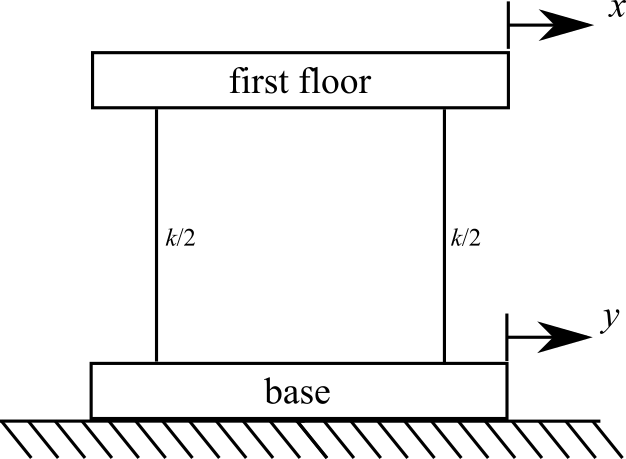
\includegraphics[width=0.35\textwidth]{../../Figures/base_excited_structure.png}
			\end{figure}				
						
			\textbf{Solution a)}
				
			For simplicity, we can rearrange the system as what follows:
			\begin{figure}[H]
				\centering
				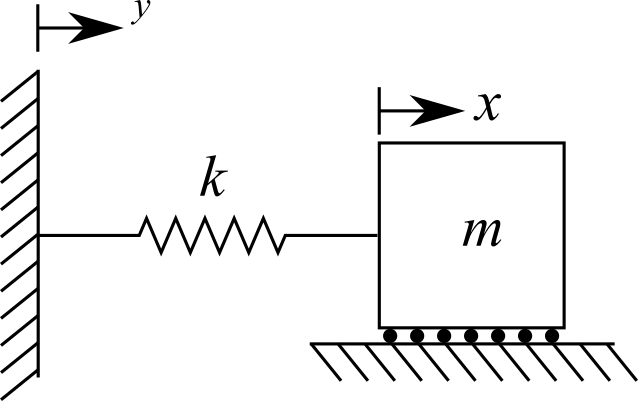
\includegraphics[width=0.35\textwidth]{../../Figures/base_excited_structure_simple.png}
			\end{figure}			

			solving for the EOM yields:
			\begin{equation}
				m\ddot{x} + kx = ky
			\end{equation} 				
			Notice that this is the same as the EOM for a damped 1-DOF system if $c=0$.	
			\begin{equation}
			m\ddot{x} + c\dot{x} + kx = + c\dot{y} + ky \rightarrow m\ddot{x} + kx = ky
			\end{equation}
			Therefore, we can use the solution:
			\begin{equation}
				x_p(t) = 	\omega_n Y   \sqrt{\frac{\omega_n^2 + (2 \zeta \omega_b)^2 }{(\omega_n^2 - \omega_b^2)^2 +  (2\zeta \omega_n \omega_b)^2} }  \text{cos}(\omega_bt - \phi_1 - \phi_2)
			\end{equation}
			where:
			\begin{equation}
				\phi_1 = \text{tan}^-1\bigg(\frac{2\zeta \omega_n \omega_b}{\omega_n^2 - \omega_b^2}\bigg)
			\end{equation}	
			\begin{equation}
				\phi_2 = \text{tan}^-1\bigg(\frac{\omega_n}{2\zeta \omega_b}\bigg)
			\end{equation}
			Now we have, or can easily get, values for $\omega_n$, $\omega_b$, and $\zeta$. However, we do not have an expression for $Y$. We can extract the displacement (and therefore the $Y$) from the acceleration as:
			\begin{equation}
				\ddot{y}(t) = A \text{cos}(\omega t)
			\end{equation} 				
			\begin{equation}
				\dot{y}(t) = \frac{A}{\omega} \text{sin}(\omega t) + C_1
			\end{equation} 					
			\begin{equation}
				y(t) = - \frac{A}{\omega^2} \text{cos}(\omega t) + C_1t + C_2
			\end{equation} 					
			Resulting in 
			\begin{equation}
				Y = -\frac{A}{\omega^2}
			\end{equation} 			
			
			\textbf{Solution b)}
			From the plots we solved for before, we can see that we want a critical damping coefficient that is as low as possible. This means any damping added to the system will decrease its safety. This may seem counter-intuitive, but this is because we are attempting to drive the structure at a frequency higher than its natural frequency, something that does not commonalty happen. Typically excitations for a structure are well below its natural frequency.  			
			
			
				
\end{document}


























